\scanpage{201}
\[
\begin{aligned}\tau_f+\tau_{f'}&=\Sigma_a\\\tau_{f'}+\tau_{f''}&=\Sigma_{a'}\end{aligned}
\quad\longrightarrow\quad
\tau_f-\tau_{f''}=\Sigma_a-\Sigma_{a'}=\Sigma_{\bar a}-\Sigma_{\bar a'}
\]
i.e.\quad $\Sigma_a+\Sigma_{\bar a'}=\Sigma_{a'}+\Sigma_{\bar a}$

\figure{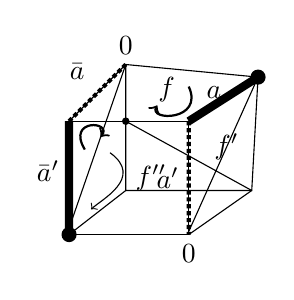
\begin{tikzpicture}[scale=.8]
\draw (0,1.8)--(1.9,1.8)--(1.9,0)--(0,0)--cycle;
\draw (.9,2.7)--(3,2.5)--(2.9,.7)--(.9,.7)--cycle;
\draw (0,1.8)--(.9,2.7) (1.9,1.8)--(3,2.5) (1.9,0)--(2.9,.7) (0,0)--(.9,.7);
\draw[line width=3pt] (0,0)--(0,1.8) (1.9,1.8)--(3,2.5);
\draw[densely dotted,line width=1.5pt] (0,1.8)--(.9,2.7) (1.9,1.8)--(1.9,0);
\draw (0,.1)--(.9,2.7) (1.9,.05)--(3,2.5) (.9,1.8)--(2.9,.7);
\fill (0,0) circle(.12);\fill (3,2.5) circle(.12);\fill (.9,1.8) circle(.06);
\node[above] at (.9,2.7) {$0$};\node[below] at (1.9,0) {$0$};
\node[above left] at (.4,2.3) {$\bar a$};\node[left] at (0,1) {$\bar a'$};
\node[above] at (2.3,2) {$a$};\node[left] at (1.9,.9) {$a'$};
\node at (1.55,2.3) {$f$};\node at (1.3,.9) {$f''$};\node at (2.5,1.4) {$f'$};
\draw[->,thick] (.25,1.35)..controls (-.05,1.85) and (.7,1.8)..(.5,1.55);
\draw[->,thick] (1.9,2.35)..controls (2.15,1.8) and (1.25,1.8)..(1.4,2.05);
\draw[->] (.65,1.3)..controls (1.2,.9) and (.5,.55)..(.35,.4);
\end{tikzpicture}}
\[\Sigma_a+\Sigma_{\bar a'}=\Sigma_{a'}+\Sigma_{\bar a}\]
\[4\cdot3\cdot2=24=48/2\]
\[
\begin{aligned}
\tau_f+\tau_{f'}&=\Sigma_a&\qquad
\tau_{\tilde f}+\tau_{\tilde f'}&=\Sigma_{\tilde a}=\Sigma_a\\
\tau_f\tau_{f'}&=\Pi_a&
\tau_{\tilde f}\tau_{\tilde f'}&=\Pi_{\tilde a}=\Pi_a
\end{aligned}
\]
donc $\{\tau_f,\tau_{f'}\}=\{\tau_{\tilde f},\tau_{\tilde f'}\}$

\figure{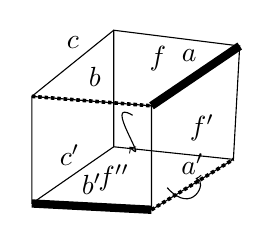
\begin{tikzpicture}[scale=.8]
\draw (0,1.8)--(1.9,1.65)--(1.9,0)--(0,.1)--cycle;
\draw (1.3,2.85)--(3.3,2.6)--(3.2,.8)--(1.3,1)--cycle;
\draw (0,1.8)--(1.3,2.85) (1.9,1.65)--(3.3,2.6) (1.9,0)--(3.2,.8) (0,.1)--(1.3,1);
\draw[line width=3pt] (1.9,1.65)--(3.3,2.6) (0,.1)--(1.9,0);
\draw[densely dotted,line width=1.3pt] (0,1.8)--(1.9,1.65) (1.9,0)--(3.2,.8);
\node[above] at (.65,2.4) {$c$};\node[above] at (1,1.8) {$b$};
\node[above] at (2.5,2.2) {$a$};\node[above] at (2.55,.4) {$a'$};
\node[above] at (.6,.55) {$c'$};\node[above] at (.95,.08) {$b'$};
\node at (2,2.4) {$f$};\node at (2.7,1.3) {$f'$};\node at (1.3,.5) {$f''$};
\draw[->] (1.6,1.5)..controls (1.1,1.8) and (1.9,.65)..(1.55,1);
\draw[->] (2.15,.35)..controls (2.55,-.1) and (2.8,.45)..(2.6,.5);
\end{tikzpicture}}
\[
\left.\begin{aligned}
\tau_f-\tau_{f''}&\unsure{=|-}\Sigma_a-\Sigma_{a'}=\Sigma_b-\Sigma_{b'}\\
\Sigma_a+\Sigma_{b'}&=\Sigma_b\unsure{\cdot|+}\Sigma_{a'}
\end{aligned}\right\}\quad\text{donc}\quad
\begin{gathered}\tau_f=\tau_{\tilde f}\quad\text{\textcircled{ou}}\\
\tau_f=\tau_{\tilde f'}\end{gathered}
\]
\figure{\begin{tikzpicture}\draw (0,0)--(6,.55);\end{tikzpicture}}
\[
\begin{aligned}
\Sigma_a-\Sigma_{a'}&=\Sigma_c-\Sigma_{c'}\\
\Sigma_a+\Sigma_{c'}&=\Sigma_c+\Sigma_{a'}
\end{aligned}
\]
$\Sigma_a$ ne dépend que de la direction de $a$

donc \uline{il n'y a que trois valeurs} de $\Sigma_a$

de même il n'y a que trois valeurs de $\Pi_a$

\figure{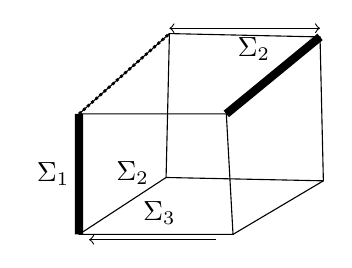
\begin{tikzpicture}[scale=.85]
\draw (0,1.8)--(2.2,1.8)--(2.3,0)--(0,0)--cycle;
\draw (1.35,3)--(3.6,2.95)--(3.65,.8)--(1.3,.85)--cycle;
\draw (0,1.8)--(1.35,3) (2.2,1.8)--(3.6,2.95) (2.3,0)--(3.65,.8) (0,0)--(1.3,.85);
\draw[line width=3pt] (0,0)--(0,1.8) (2.2,1.8)--(3.6,2.95);
\draw[densely dotted,line width=1pt] (0,1.8)--(1.35,3);
\draw[<->] (1.35,3.08)--(3.6,3.08);\draw[->] (2.05,-.08)--(.15,-.08);
\node[left] at (0,.9) {$\Sigma_1$};\node[above] at (.8,.6) {$\Sigma_2$};
\node[above left] at (3,2.45) {$\Sigma_2$};\node[above] at (1.2,0) {$\Sigma_3$};
\end{tikzpicture}}
$12$ relations de la forme $\Sigma_a+\Sigma_{a'}=\Sigma_b+\Sigma_{b'}$

\deleted{pour $\Sigma_a$ fixé}
Via opération du groupe symétrique $\mathfrak S_4$, elles se déduisent l'une de l'autre
\margin{200}
